\chapter{Methodology}
\section{Introduction}
Cyberspace is the digital creativity environment in which we live and
which is controlled by cybersecurity.  Perhaps the basic vision of
cybersecurity is to reach a \emph{virtuous} digital world.  In order to
reach such a strategic goal, the mission of cybersecurity must be how
to insert human ethics and values into software values.  This matter
in itself is not easy at all because it requires an ethical philosophy
related to cybersecurity.  This philosophy proposes that cyberspace
be an \emph{ideal} alternative to the real world as much as possible.
What we mean by \emph{idealism} here is that the presence of each member
in this space is effective and not harmful to others.  To achieve this
requires answering two important questions.

\begin{enumerate}
\item What is the current presence of members in cyberspace? And,
\item how can this presence be digitally enhanced to be ideal?
\end{enumerate}

Through this chapter, we tried to provide a convincing answer to both
questions by developing a  logical framework for cybersecurity. 
%that proposes stakeholder policies and a social contract of cyberspace.



\section{Logical analysis}
%-------from hand book-ch1-1.3 Methodology begin
Although the science and art of computing, and of communication, form the foundation on which cybersecurity rests, we cannot use these disciplines to explain or unlock the mysteries of cybersecurity. Also, much as number theory has a special place in the world of cybersecurity, it does not provide skills or ideas of the sort that are relevant regularly to cybersecurity professionals. But there is an area of mathematics that is relevant to almost every attack, not just upon encrypted communication, but all cyber-attacks. 

This area is {\em logic}. The concept of {\em logic} is relevant to everyone, and all fields of human endeavour. The importance of logic is imposed, by reality, by anyone who ignores it. Conseqently, everyone has a basic understanding of logic. What varies, from one to another, is not so much understanding of logic, as awareness of when it is in use. Not everyone is self-conciously {\em aware} when they are using logic.

This extra step of {\em self-aware application} of logic is not always necessary but helps in cases of critical importance, where getting details wrong can sometimes cause serious harm. In cybersecurity, as in pure mathematics, the consequences of minor logical mistakes can sometimes be disastrous. 

This is why, in this dessertation, {\em mathematical} logic is regarded as the key scientific method which we employ to analyse cybersecurity problems, and in the design of cybersecurity solutions.
\if
This is not meant to suggest that mathematical logic should be used on a regular basis by cybersecurity professionals. Many cybersecurity professionals will never use it, and currently, many may not even have heard ot it. However, {\em logic} is used by all cybersecurity professionals on a regular basis. In the course of understanding how this takes place, and how it is done consistently and correctly, with as little chance of error as possible, we need to develop the sort of self-awareness, of what we are doing, that is best characerised, and explained, in the particular form of logic known as mathematical logic.\index{logic!mathematical}
%-------from hand book-ch1-1.3 Methodology end
\fi
[One of the methods used in this work is to apply logic to cybersecurity objectives. 

In particular, logic can be used to show {\em how} cybersecurity objectives can
be met. Logic is the appropriate tool, for example, if the objective sought can
be shown to follow, logically, from certain other rules.

In some cases it may also be possible, and useful, to show that certain objectives can {\em only}
be met in certain ways.]

In this section, we developed concepts and tools which assist cybersecurity professionals to define the mandatory objectives of their systems, the rules which enforce these objectivities, and the reasoning behind the choice of these rules. The concepts and tools we proposed and illustrated in this section will be shown, in Chapter 5, to be sufficient to record and analyse these rules, both the objectives and the rules which are enforced, and to ensure that there are no logical flaws in the system which has been designed. Note that we assume our cybersecurity objectives include the control of all important risks. 
\subsection{cybersecurity architecture}
The concept that cybersecurity architecture is the discovery, definition and validation of {\em rules} (mandatory objectives and their conditions) is introduced.

\subsection{Inference graphs}\label{inferencesec}
The new concept of {\em inference graphs} for illustrating the relationship between cybersecurity rules is defined. The collection of cybersecurity rules forms a graph, in which the vertices represent cybersecurity rules, and the edges represent {\em inference}, in the sense that the collection of vertices with edges {\em terminating} at a certain vertex, $V$ for example, correspond to the set of rules which are sufficient to prove the rule corresponding to $V$. This representation of cybersecurity provides a way to develop cybersecurity architecture\cite{Rerup2018}. These diagrams can also be used in security design, as a way to validate security designs, for documentation, and as a way to visualise and develop alternative designs.

An inference graph shows the relationship of {\em inference} (what implies what) which applies to the different cybersecurity rules which apply in a system.
Examples of inference graphs are shown in Figures \ref{parcelboxrules}  and \ref{certificaterulesgraph}. These will be explained in Section \ref{examplesec}.

The following types of rules arise in cybersecurity analysis: {\em objective}, {\em enforced rule}, {\em axiom}, {\em proposition}, and {\em assumption}. An objective is a rule which is required to be true at all times. An enforced rule is a condition that is possible to enforce, and which it has been decided to enforce, by technical means. For example, access to many systems is only provided if a user is able to enter a valid username and password.

An axiom is a condition that is held to be true {\em a priori}; an assumption is a condition which we {\em choose} to believe. For example, under some conditions, we assume that users do not reveal their password to other users. A proposition is a rule or statement which we define in order to express a useful stage of reasoning.

An {\em edge} in an inference graph connects each of the rules referenced in proof to the rule which is proved. Objectives are typically the destination of edges, while enforced rules usually occur only as of the origin of an edge.

\subsubsection{Proof as a relationship}
The {\em goal} of cybersecurity is to guarantee that certain objectives are maintained. For example, it is likely that a bank will have, as an objective, that no transactions -- transfers of money from one account to another -- occur except with valid authorization.

The aim of cybersecurity {\em design} is to discover or instantiate axioms, assumptions, and enforced rules which enable us to {\em prove} that the {\em objectives} are true. Along the way to doing this, there may be some {\em intermediate propositions} that we also wish to prove.

Thus, {\em objectives} and {\em intermediate propositions} have proofs. On the other hand, {\em axioms} do not have proofs because these are fundamental truths that are true from logical principles or, in some cases, because they express follow from the definition of the predicates they contain, {\em assumptions} are true by assumption (which might not always hold, but at present we adopt them), and {\em enforced rules} are true because we make sure, in the system, that they are true, so none of these rule types has proofs.

The appearance of a reference to a proposition, assumption, axiom, objective, or enforced rule, in a proof,  constitutes a relationship between that rule and the rule is proved. The {\em inference graph} has vertices or nodes corresponding to the rules and directed edges or links from any rule which is referenced in proof to the rule which is proved.


In the diagrams which are included below, the different types of rules are represented by nodes of different shapes and colours, as  indicated in the Legend, shown in Fig. \ref{legend}. \begin{figure}[bhpt]
	\centering
		\leavevmode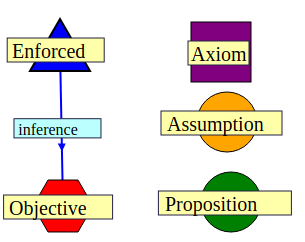
\includegraphics[width=42mm]{legend.png}\ \\
		\caption{Legend for Inference graphs}\label{legend}
\end{figure}




\subsection{Examples of inference graphs}
Three increasingly complex examples of inference graphs for systems needing cybersecurity architecture are presented, including the detailed proofs which form the basis of these inference graphs, in some cases. 

We see how a key design objective is achieved rigorously by a clever decision that emerges from the use of the cybersecurity inference graph of this system. Example 2 is based on a cybersecurity weakness in a web service administered by one of the authors, which was analysed and solved previously \cite{exptsandproofs} so in this case, the inference graph is used to illustrate the proofs which were developed then. In Example 3, finding the correct proofs was a complicated task which was facilitated by the use of the inference graph of rules and objectives of the system.}



\subsection{Inference Graphs Software}
 
The software which has been developed to support the development and use of cybersecurity inference graphs is described including details of the public server where it can be used. 

\subsection{Conclusion}
In this section and Chapter 5, we tried to show that cybersecurity inference graphs can significantly contribute to the development of, and validation of cybersecurity and also that rigorous validation of cybersecurity is not necessarily as complex as previously thought.

\section{Experiments using examples}
\iflonger
\subsection{security audit}
An approach used periodically is to assign the task of attack or harm   a service in cyber space  to an individual or a team and then address the discovered weaknesses. We call this a {\em security audit}. The approach of searching for weaknesses and fixing them is so widely used that it might reasonably be regarded as a design philosophy.
This approach has been used in this dissertation, and the results of
both the attacks and the resulting defences are reported.
However, this approach is somewhat pessimistic in that it {\em assumes}
that a more methodical security design philosophy which can guarantee
secure design is not available.
\fi

\section{Gathering ideas and reviewing ideas from literature}


An important methodology in this dissertation, as in all scientific work, is to gather the thoughts of other researchers, who are struggling with the same problems as tackled here, and to identify key ideas and principles that have previously been suggested, and to recognise the most important of these and make use of them in this work.
\if
Because web services (including services provided via apps on mobile phones)
are a recent development and continue to evolve in both details and fundamentals,
principles of secure design of these services is also a new and evolving area of
research and development \cite{AddieColman2010,Addie_Moffatt_Dekeyser_Colman2011}.
\else\cite{Addie_Moffatt_Dekeyser_Colman2011}.
\fi

This section reviews three different approaches for securing web sites/services.
Each of these approaches is usually expressed as a completely independent
philosophy for achieving good security. We shall see that these approaches 
are actually complementary, and to achieve rigorous security all three approaches
are needed. Note that although we describe a design philosophy which is able, formally, to prove,
i.e.  guarantee, security, because no logical system can claim certainty in an absolute
sense (in mathematical logic, this fact is expressed in G\"odel's incompleteness theorem), the strategy 
of attacking the system remains useful, even after it has been
methodically proved to be correct.

The present paper does not apportion equal emphasis on all approaches
because the original contribution of this paper is 
in the third of them, together with the way the second approach joins
with the third to form a more comprehensive whole. The second approach
is the one summarised in Subsection \ref{audit} and applied
in Section \ref{expts}.
The third approach is summarised in Subsection \ref{stsecanal} and applied
to the Netml password reset system in Sections \ref{stakeholders} and \ref{proof}.

%\subsection{Web Service Security Design}\label{webservicessecurity}







\subsection{Good Security Design Practice}
Good design takes security, ease of access, and usability into account,
striking a balance between protecting the system and ease of use. Good
practice has evolved a number of practical approaches like  minimizing
attack surface area \cite{bhardwaj2018reducing},  establish secure
defaults \cite{lai2018impact}, using the principle of defence in depth
\cite{toch2018privacy}, not trusting services \cite{ghirardello2018cyber},
keeping security simple \cite{thomsen2018network}, and fixing security
issues correctly \iflonger\cite {ali2018security, tabassum2018evaluating}.
\else \cite {tabassum2018evaluating}.\fi
These approaches  are used for  maintaining and improving security which
are so natural and important that they should be adopted as a first
layer of protection as a matter of standard practice, even when more
sophisticated approaches are also in use \cite {ross2018systems}.


\subsection{Security Auditing}\label{audit}

Strategies for breaking into web systems or services are under continuous
development by government and non-government organisations and individuals,
both those with friendly intentions and those who wish to exploit security
weaknesses for their own advantage. When
a new exploit is discovered, if it is discovered first by those with 
friendly intentions, defences against the exploit are usually developed
quickly and published. Exploits discovered by attackers with ill intent
can, of course, be deployed before web managers have the opportunity
to defend against them. Also, in the period of time immediately after
the defence against a new exploit has been published, there is still
an opportunity to attack web sites which have not deployed the newly developed
defences. This time can be somewhat extended due to the limitated expertise
of web-site owners and because the sequence of steps required to address a weakness
in a high-level framework can be quite lengthy.

A widely used strategy for improving web site or web service security is
to attempt to attack the site by using the strategies which are currently
known to be effective one-by-one, or simultaneously, to discover if the
site is vulnerable to any of these strategies. Since all of the strategies
tried are known, the defences against all of them are also almost certainly
known, and hence can be adopted by the web site.

Experiments of this type, and the resulting web service design improvements,
are described in Section \ref{expts}.



\subsection{Stakeholder Security Analysis}\label{stsecanal}

A more fundamental strategy which is not well-developed at present is
to seek to develop provably secure protocols and software for all aspects
of a web service \cite{whitman2011principles,mailloux2018examination,bishop2005introduction}.

The first step in this approach, which is developed further in 
Section \ref{stakeholders}, is to consider the point of view of all legitimate stakeholders
in relation to the service, and to enumerate a complete set of rules
required by each of these stakeholders, sufficient to ensure that they
will agree to actively participate in the service.


\section{Stakeholder Security Analysis}

[Stakeholder security analysis is a more specific form of logical analysis. Instead of dealing with
objectives in general, it makes use of the obvious but useful fact that all systems have
stakeholders, and the objectives of the system as a whole can be sub-divided into those
which can be ascribed to each stakeholder. Once their objectives have been identified, they
can be further analysed, refined, and reviewed. In particular, it is important to work out if
their objectives are compatible.]
The main result of this dissertation is to demonstrate  a secure methodical design philosophy.
We call this {\em stakeholder security analysis}.

%Hand book-----ch2-2.3.1 begin
Every business, organization, or community has {\em stakeholders}. These are the people (or agents) who have an interest in any aspect of its operation. In many cases, there will be a large group of {\em clients}, i.e. individuals who receive a service. There may be one or more {\em owners}. There are also many other ways a person, agent, or entity can have an interest in a given organisation or entity. One organization can be a stakeholder in another.
%Hand book-----ch2-2.3.1 end

In this section, we designed stakeholders' policies to incorporate human
values and ethics as much as possible into software values

Stakeholder security analysis proceeds as follows: 
\begin{enumerate}[1.]
\item Identify the key stakeholders.
\item For each stakeholder, identify a set of rules {\em required}
by these stakeholders. Note: the collected rules required
by all stakeholders must be consistent.
\item Implement procedures which ensure that all rules are enforced.
\end{enumerate}

Both a security audit and a stakeholder security analysis
are applied in this dissertation to a specific subsystem of a web
service system being developed and managed by the authors.
Note: it is not suggested that stakeholder security analysis obviates
the need for a security audit.

\subsubsection{Stakeholder Roles}\label{strol}
The roles are defined first, then their stakeholders, and access levels and features are set in those roles. Security rules are defined based on stakeholders roles, and not stakeholders themselves, where we can state the rule in terms of anyone who is playing a certain role. Stakeholder experiences should be shared to identify vulnerabilities that may occur while dealing with the service or part of the system under study. Most organizations consider the reputable more than the performance of their systems. Therefore, they adopt robust security solutions. However, access levels for sources as well as sensitive data often require additional restrictions above standard security requirements. Hence,  additional restrictions are identified and chosen with extreme care, ensuring their independence, and providing sources and data to the real interest without any other party who can access the current security restrictions.
\subsubsection{Stakeholder Business Rules}\label{stbsnrul}
Business rules refer to any rule relating to the way in which transactions are restricted. Business rules must be observed when designing and improving system security. In other words, even if the proposed security rules are enforced, they must be considered to be subject to the satisfactory standard by their professional organization. It is necessary to focus on Business rules  which are explicit rules on safety and try to study them and analyze them before drafting the security rules to avoid the contradiction.
The expectations of stakeholders which constitute a security case are considered mandatory and must be included in a security rule.

\subsection{Stakeholders}

Every business, organization, or community has {\em stakeholders}. These are the people (or agents) who have
an interest in any aspect of its operation. In many cases there will be a large group of {\em clients}, i.e. 
individuals who receive a service. There may be one or more {\em owners}. There are also many other ways
in which a person, agent, or entity can have an interest in an a given organization or entity. One organization
can be a stakeholder in another.

\subsection{Stakeholders Rules}

Any business, organisation, club or association has {\em stakeholders}. A stakeholder is a person, or 
entity, with some interest in activities of the organisation. Typically, there will be 4-5 key stakeholders.

\begin{sbexample}{Stakeholders of a University}%
Consider a university, for example. Key stakeholders are: (i) students, (ii) staff (which may be further
subdivided into academic, administration, management, and support staff), (iii) employers of graduates,
(iv) governments, and (v) parents of students.
\end{sbexample}

Many of the rules expected or mandated by stakeholders fall into fairly standard categories, like
{\em legal requirements}, {\em ethics}, etc, which are fairly similar across different stakeholders.
Most of these requirements are well-known, but nevertheless, these requirements do call for 
rules that need to be enforced by security design. Therefore it is useful for us to consider these
requirements explicitly. We consider these generic rules first.

\subsubsection{Specific Stakeholder Rules}

Stakeholders of an institution have certain reasonable expectations that are
probably understood by the other stakeholders, or which they communicate to them
either explicitly, or by their actions. Many of these expectations will lead
to rules that are explicitly or implicitly imposed on the operation of the institution.

\begin{sbexample}{Stakeholder Rules for a University}%
Continuing with the previous example, let us explore the rules that the stakeholders of a university
expect (or insist) should hold.

{\bf Students}

Students enrol and attend university to receive an education. They expect this education to qualify
them to gain work in their field of study. 

In addition, students have reasonable expectations regarding their ability to succeed or excel.
They expect to be able to make use of and learn by means of the learning resources provided to
them, to be able to achieve better results by spending more time and focussing more effectively
on their studies. They expect their efforts to be rewarded fairly, relative to other students.
In particular, they expect students with poor understanding, or who attempt to succeed without
really engaging in the learning process in an effective or legitimate way to be identified and
to achieve significantly worse outcomes.



{\bf Staff}

Staff expect to receive satisfactory remuneration for their work, to be adequately resourced,
including satisfactory computing, and communication resources. They also expect their managers
to provide adequate guidance concerning their resonsibilities, and training to enable them
to complete their responsibilities with a high level of professionalism.


Staff expect records concerning themselves to be treated with appropriate care, and in particular,
such records should not be shared with others except for purposes which are reasonable and 
with which they are in accord.

{\bf Employers}

Employers expect graduates from a university to be able to communicate, and collaborate with
other employees. They expect graduates to behave ethically (and in particular, honestly) in relation
to their work, employer, clients and colleagues. The also expect graduates to have knowledge
and understanding in the technical area in which they were studying.

{\bf Governments}

Governments expect students to receive an education which enables them to gain employment and
make a sound contribution to their employers. They expect university staff to act with respect and
probity toward each other, and toward students.

{\bf Parents}

Parents expect universities to treat their children with respect, to provide them with 
a good education, assessed fairly, and without subjecting them to harrassment or
abuse of any kind.

\end{sbexample}

Much of what stakeholders expect and demand cannot actually be encapusulated in a {\em rule}.
This doesn't mean that we should ignore such expectations. However, these expectations
are not usually considered relevant to {\em cyber-security}. In general, it is only
the expectations which are a matter of insistence, i.e. these are mandatory requirements,
which we consider to be an issue of security.


\iffalse
\subsubsection{Stakeholder SWOT}\label{stswot}
The SWOT analysis tools are used to evaluate the security aspects for the stakeholders in the system Fig(). The first step is to determine the security objectives required by each stakeholders role and business rules within the specific service,Password Reset Service. And then identify the internal factors (strengths, weaknesses) and external factors (opportunities, threats) that are favourable and unfavourable to achieve those objectives.

Strengths are an opportunity to support security objectives, while weaknesses are considered to be the vulnerabilities that may impede the achievement of these objectives. The statement of the risks of weaknesses and the great efforts to fix them and clarify the strengths in the implementation of the security rules that prevent such circumstances are sufficient justification for obtaining the approval of the owners of the decision. On the other hand, the lack of funds and inconsistencies with business rules in achieving security objectives are weaknesses. In terms of opportunities, they are any initiatives available to support security objectives such as sources, expenditures, technologies, and security policies.Threats are related to the importance of the system and the sensitive information it contains. They often exploited weaknesses.


%These objectives support the protection of password reset service.
\subsubsection{Stakeholder Security Rules}\label{stsecrul}
\subsubsection{Assumption}\label{assmp} 
After completing security rules, assumptions are developed that simplify the logic necessary to complete the design process. The degree of simplification is determined depending on the sensitivity of the security issue. Security rules are therefore classified as optional or mandatory. Unlike the optional category, which is assumed or obvious assumptions, mandatory class assumptions are security requirements that need to be adopted in the design or development of system security.
\subsection{Stakeholder Security Design}\label{stsecdsgn} 
The main goal in the design phase is to know which of the mandatory security rules must be guaranteed and how to do it. When a particular  rule is not guaranteed directly,  this rule should be checked  that it follows from our assumptions and the rules which are enforced. However , there are three categories of rules: (i)assumptions; (ii) enforced rules; (iii)rules that must be proven, and through careful examining of the latter, the process of checking security becomes more reliable and systematic.

In addition, unrealistic assumptions may cause security vulnerability. Also, very strict assumptions can undermine security. However, the combination of the two methods can lead to simple and effective security design and achieve a higher security level in certain situations of critical importance.
\subsubsection{Inforcable Stakeholder Security Rules}\label{Instsecrul}
\subsubsection{Validation of Stakeholder Security Rules}\label{vlstsecrul}

[It is not always possible to prove hypotheses, even when there are strong reasons for believing
them to be true. In science, and even in mathematics, some valid hypotheses can only be demonstrated
by examples. A very good example of this sort of hypothesis is Church's thesis, which is that
all concepts of computability are equivalent to Turing computability. A very large number of papers
were written, in the past, which showed that this or that type of computability was equivalent to
Turing computability. Eventually, journals put a stop to such publications. The concept that there is
really just one type of computable function had been established. But it was not a provable concept.
It was necessary to prove it by examples.

There are other advantages of examples. They are also an ideal way to demonstrate ideas in a 
natural and attractive fashion.

In this dissertation, many examples will be used to illustrate ideas which are in an obvious
sense quite similar in multiple superficially different cases. The striking similarity, in
different contexts, demonstrates that the concept is not an accident, but represents an important
principle.]




\iffalse
\section{A social contract for cyberspace}
We proposed a social contract for cyberspace that can manage Stakeholders'
policies and ensure their respect by their owners.
\fi

\fi